\clearpage
\subsection{Design}

\subsubsection{scope}
\par{This section provides the details use case requirements for the use cases offered by the Design
module.}

\begin{figure}[h]
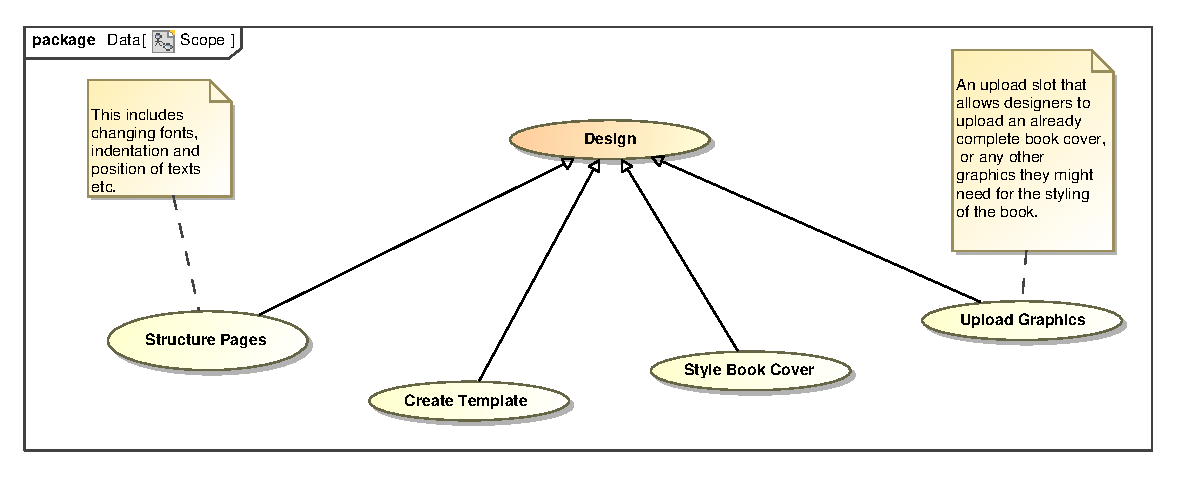
\includegraphics[scale=0.5]{epsImages/Design/Scope.eps}
\caption{Scope of Design module}
\end{figure}

\subsubsection{Use Cases}
\begin{enumerate}
\item \textbf{Structure Pages - priority: critical}
\par{This use case which allows one to structure the  manuscript.}
\par{\textbf{service contract:} Below is the service contract for structuring a manuscript.
}
\begin{figure}[h]
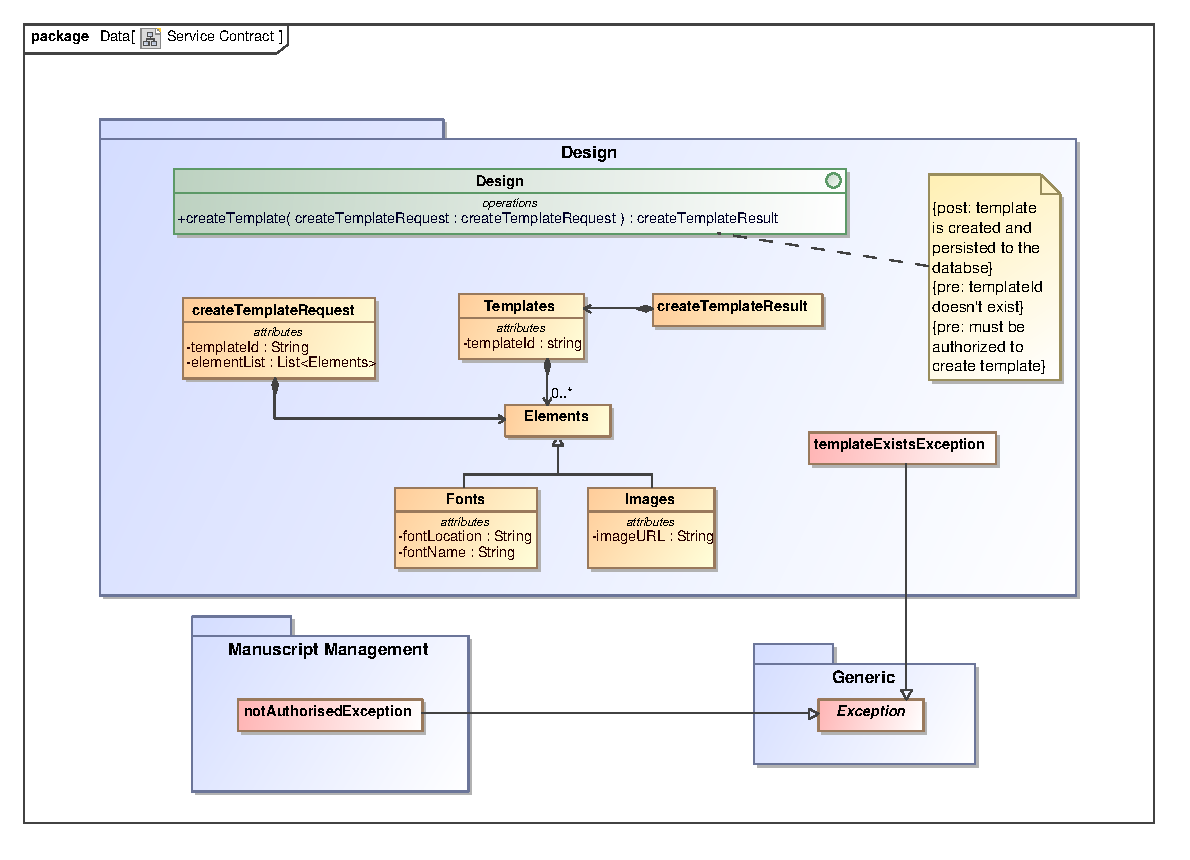
\includegraphics[scale=0.5]{epsImages/Design/createTemplateServiceContract.eps}
\caption{Service contract for structuring a menuscript}
\end{figure}

\item \textbf{Create Template - priority: nice to have}
\par{This module allows a user to create a template design for the book.}
\par{\textbf{service contract:} Below is the service contract for creating a template.
}
 \begin{figure}[h]
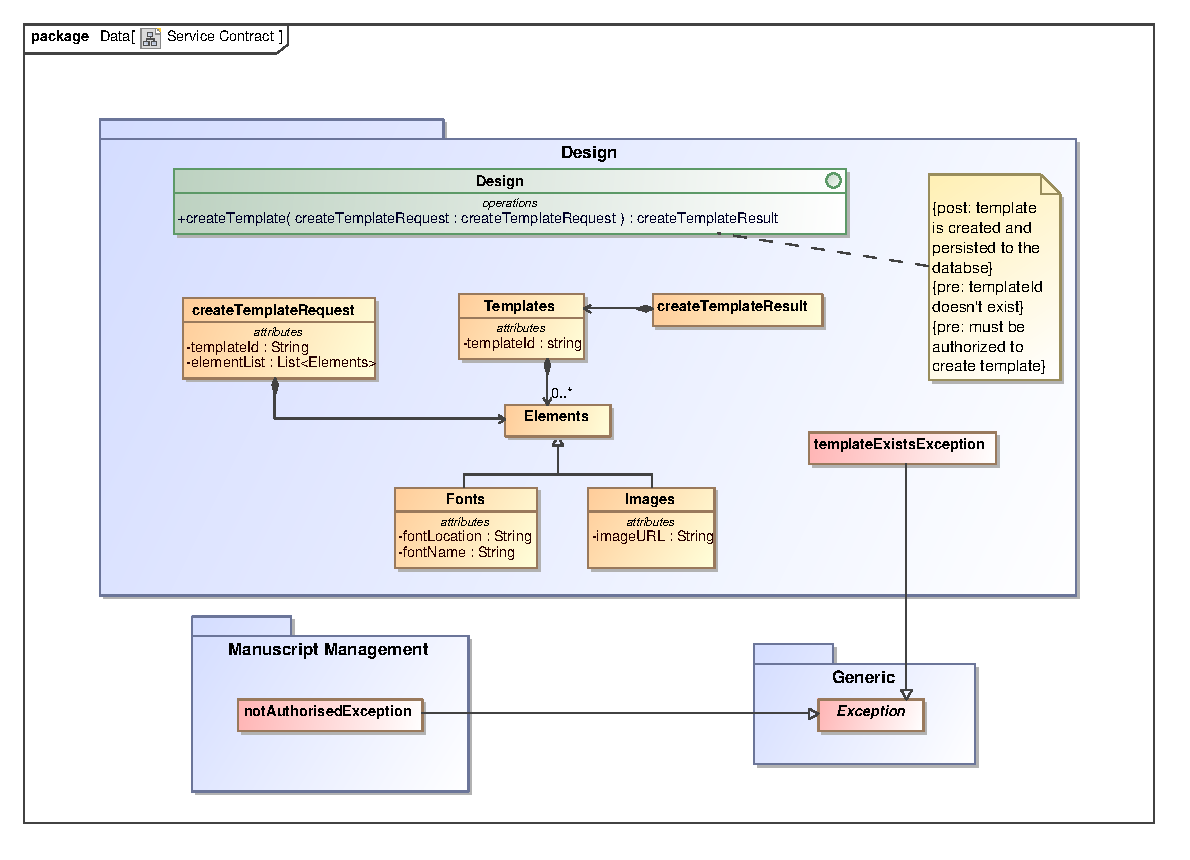
\includegraphics[scale=0.5]{epsImages/Design/createTemplateServiceContract.eps}
\caption{Service contract for creating a template design}
\end{figure}

\item \textbf{Create Book Cover - priority: critical}
\par{This use case which allows create a book cover for a  manuscript.}
\par{\textbf{service contract:} Below is the service contract for creating a book cover.
}
 \begin{figure}[h]
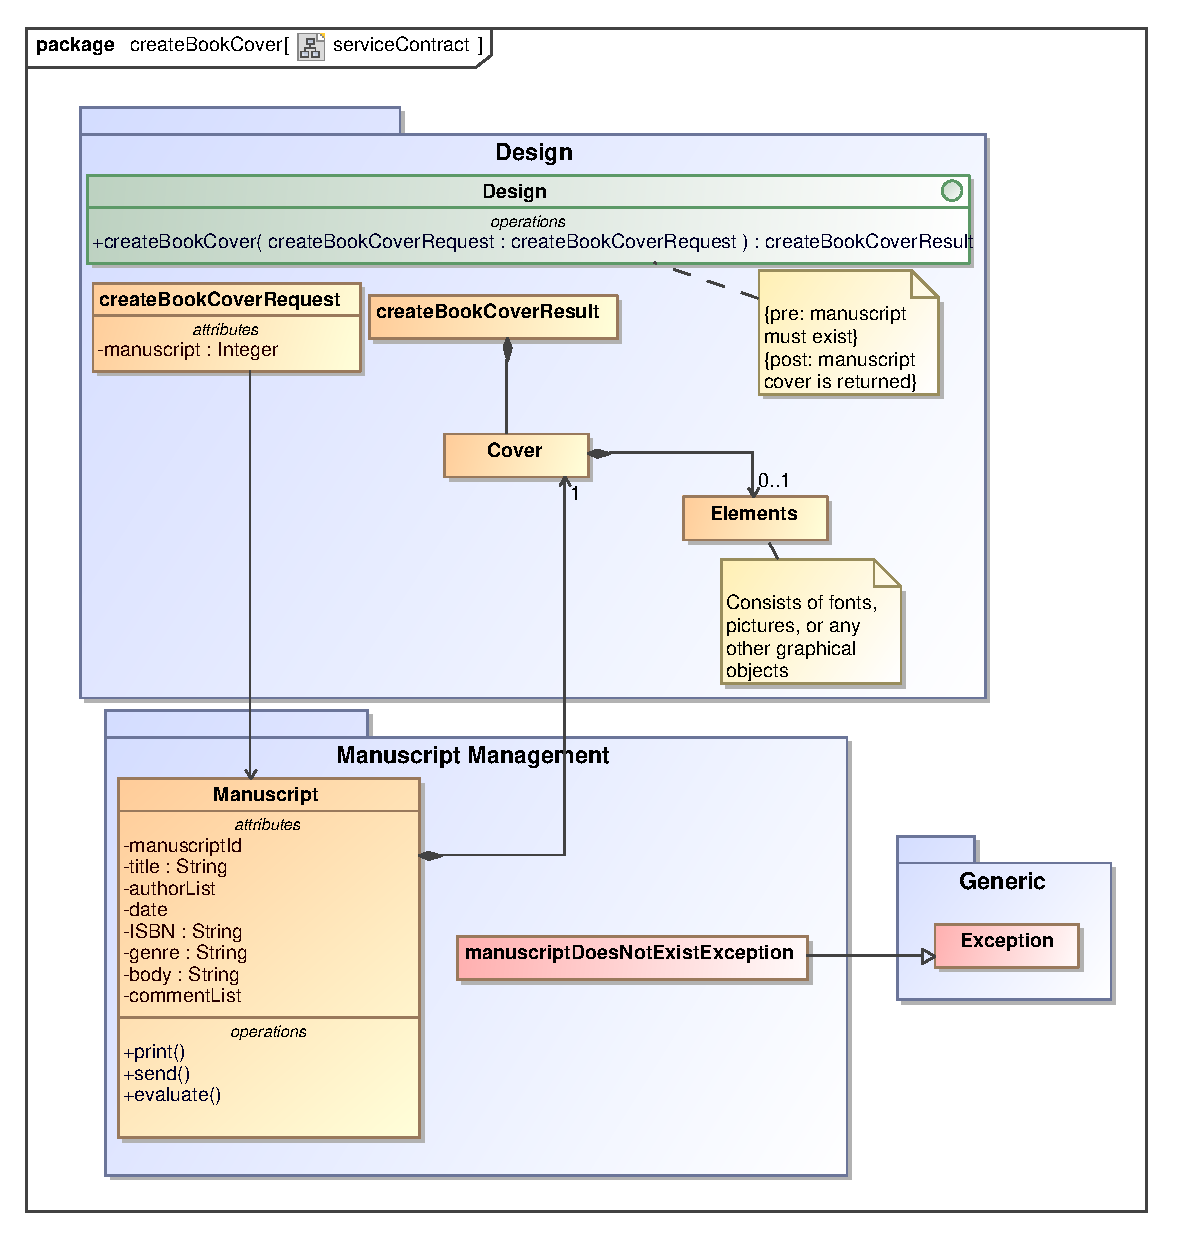
\includegraphics[scale=0.5]{epsImages/Design/createBookCover.eps}
\caption{Service contract for creating a book cover}
\end{figure}

\item \textbf{Upload Graphic - priority: important}\\
\par{This use case allows a user to open any graphic they choose. This may be a new font, or image they wish to use, or a completed cover for the book. Size and format of a graphic are restricted however.}
\par{\textbf{service contract:} Below is the service contract for uploading a graphic.
}
\begin{figure}[h]
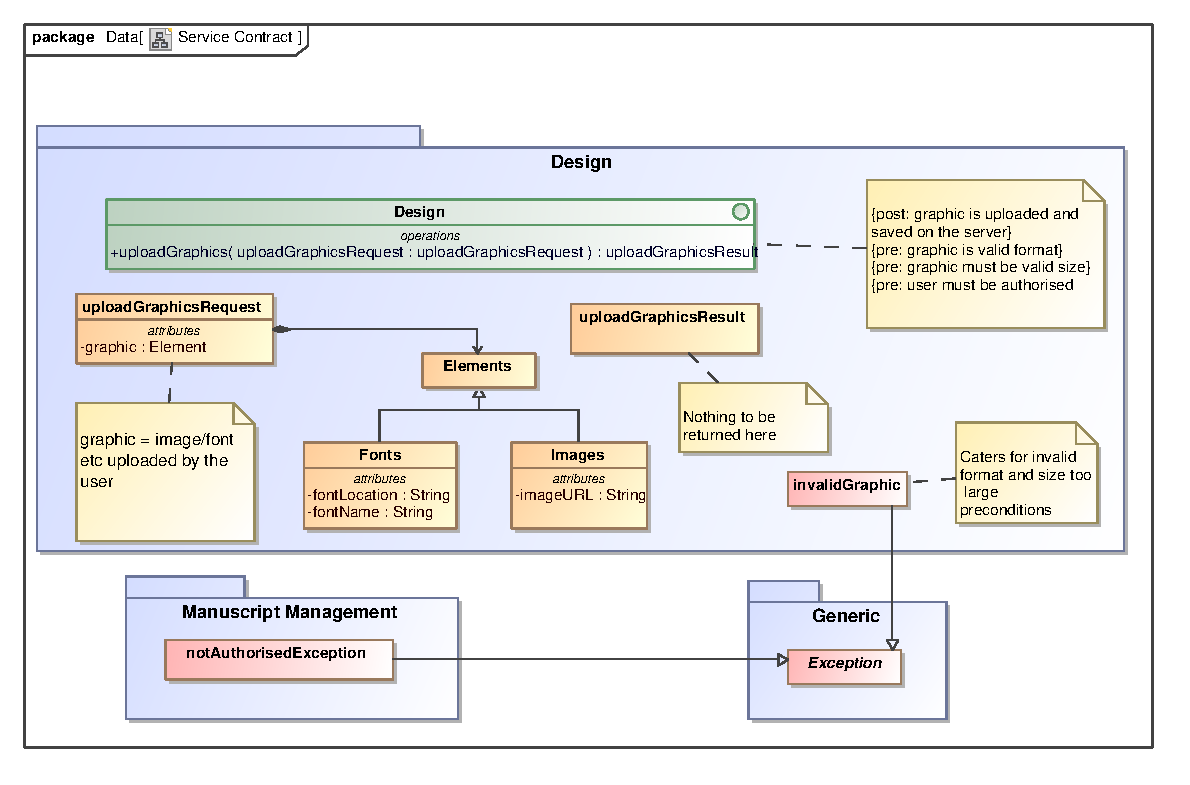
\includegraphics[scale=0.5]{epsImages/Design/uploadGraphicsServiceContract.eps}
\caption{Service contract for uploading a graphic}
\end{figure}
\end{enumerate}
